\section{Software architecture and design}
\label{chapter2}

\subsection{Software modules}

\subsubsection{Safety related modules}
\begin{enumerate}
    \item \textbf{Window Control Module (Raspberry Pi):} \\ 
        \textbf{Description:} This module receives the status (e.g., OPEN, CLOSE, IDLE) from the Communication Module and controls the electric motor to open or close the window based on the received status. It ensures safe operation by detecting obstacles or problems during movement. \\ 
        \textbf{Functions:}
        \begin{itemize}
            \item Receive status (e.g., OPEN, CLOSE, IDLE) from the Communication Module.
            \item Open/close the window using the stepper motor based on the status.
            \item Monitor motor movement and detect deviations during window operation.
            \item Stop motor and trigger an error state if a problem is detected.
            \item Report errors through LED indicators.
        \end{itemize}
        \textbf{Data:} Stepper motor position, window state, status. \\ 
        \textbf{Requirements:} \ref{req.4} (Operating the window), \ref{req.1.5} (Connection retries and email alerts), \ref{req.3.1} (Acknowledgment of messages).
        
    \item \textbf{Value Interpretation Module (Arduino):} \\ 
        \textbf{Description:} This module validates the CO2 sensor readings and determines whether the values are within a valid range. Furthermore it compares the current value with the average of the last measured values and sets the status based on that. The status (OPEN, CLOSE, IDLE) is then sent to the Raspberry Pi via the Communication Module. \\ 
        \textbf{Functions:}
        \begin{itemize}
            \item Measure CO2 concentration using the MH-Z19 sensor.
            \item Validate CO2 readings by checking for deviations from the average of previous readings.
            \item Determine status (OPEN, CLOSE, IDLE) based on validated values.
            \item Send status to the Raspberry Pi via the Communication Module.
        \end{itemize}
        \textbf{Data:} Raw sensor data, validated status (OPEN, CLOSE, IDLE). \\ 
        \textbf{Requirements:} \ref{req.2} (Invalid Value Handling), \ref{qreq.7} (Status communication).

\end{enumerate}
\newpage
\subsubsection{Security related modules}
\begin{enumerate}
    \item \textbf{Communication Module (Raspberry Pi and Arduino):} \\ 
        \textbf{Description:} This module handles the communication between the Raspberry Pi and the Arduino, ensuring secure and reliable message transmission, including handling connection retries and managing encryption keys. \\ 
        \textbf{Functions:}
        \begin{itemize}
            \item Establish Bluetooth communication between Raspberry Pi and Arduino.
            \item Implement acknowledgment of messages between devices.
            \item Handle connection retries and trigger alerts after failed retries.
            \item Implement Diffie-Hellman key exchange for secure communication setup.
            \item Perform encryption and decryption of messages using AES-CBC-128.
            \item Using HMAC for Data-Integrity and Authentication
        \end{itemize}
        \textbf{Data:} Encrypted communication data, status messages, acknowledgment messages. \\ 
        \textbf{Requirements:} \ref{req.3} (Communication between devices), \ref{sreq.1} (Spoofing and key exchange), \ref{sreq.4} (Information Disclosure), \ref{req.1.5} (Email alerts on failed retries).

    \item \textbf{System Hardening Module (Raspberry Pi):} \\ 
        \textbf{Description:} This module focuses on securing the Raspberry Pi against cyber threats by implementing firewall rules and monitoring suspicious activity. \\ 
        \textbf{Functions:}
        \begin{itemize}
            \item Manage user authentication and access control.
            \item Monitor and log suspicious activity.
        \end{itemize}
        \textbf{Data:} Security logs, access control records. \\ 
        \textbf{Requirements:} \ref{sreq.2} (Tampering protection), \ref{sreq.3}.3 (Repudiation logging).
\end{enumerate}

\subsubsection{Modules with no influence on Safety and Security}
\begin{enumerate}
    \item \textbf{Fan Control Module (Raspberry Pi):} \\ 
        \textbf{Description:} This module controls the fan based on the status received from the Communication Module. It turns on the fan when instructed and turns it off when instructed. \\ 
        \textbf{Functions:}
        \begin{itemize}
            \item Turn on the fan when receiving an OPEN status.
            \item Turn off the fan when receiving a CLOSE status.
        \end{itemize}
        \textbf{Data:} Status, fan state. \\ 
        \textbf{Requirements:} \ref{qreq.8} (Fan activation on OPEN status), \ref{qreq.9} (Fan deactivation on CLOSE status).

    \item \textbf{System Monitoring Module (Raspberry Pi):} \\ 
        \textbf{Description:} This module handles general system diagnostics like checking CPU temperature and memory usage. It ensures that non-critical parameters are monitored for optimal system performance. \\ 
        \textbf{Functions:}
        \begin{itemize}
            \item Log and monitor system health, such as CPU temperature and memory usage.
            \item Log non-critical warnings for maintenance purposes.
        \end{itemize}
        \textbf{Data:} System diagnostics logs, performance metrics. \\ 
        \textbf{Requirements:} \ref{qreq.1} (The system should be installed in an inaccessible location to ensure reliability).
\end{enumerate}

\subsection{Libraries}
The following libraries are used to interface with hardware components and to implement the functionality described above:
\begin{itemize}
    \item \textbf{MiCS-VZ-89TE Library (Arduino):} `MICS-VZ-89TE` or `SoftwareSerial` - to read CO2 data via UART from the MH-Z19 sensor and convert it into ppm values.
    \item \textbf{Stepper Motor Control Library (Raspberry Pi):} `wiringPi` or equivalent C libraries for controlling the stepper motor for window movement.
    \item \textbf{Communication Libraries:}
        \begin{itemize}
            \item Raspberry Pi: `bluez` (C library) - for managing Bluetooth communication.
            \item Arduino: `Arduino BluetoothSerial` - for establishing and maintaining Bluetooth connections.
        \end{itemize}
    \item \textbf{Encryption Libraries:}
        \begin{itemize}
            \item Arduino \& Raspberry Pi: `AESLib` for or encrypting and decrypting communication data
        \end{itemize}
\end{itemize}

\subsection{Interrupts}
\textbf{Definition of priorities:}
\begin{itemize}
    \item \textbf{Priority 1:} Communication failure detection interrupt between the Raspberry Pi and Arduino to ensure immediate action if data transfer fails.
    \item \textbf{Priority 2:} Window control interrupts for problem detection during motor operation to prevent damage.
    \item \textbf{Priority 3:} Status validation on the Arduino to ensure accurate CO2 evaluation.
\end{itemize}

\subsection{Pinout}
\begin{itemize}
    \item \textbf{CO2 Sensor (MiCS-VZ-89TE - Arduino):} Connected via UART for analog data reading.
    \item \textbf{Window Motor Control (Raspberry Pi):} Connected to GPIO pins for controlling the motor.
    \item \textbf{Fan Control (Raspberry Pi):} Connected to GPIO pins for fan activation.
    \item \textbf{Error Indicators (Raspberry Pi \& Arduino):} LEDs connected to GPIO pins for status indication.
\end{itemize}

\begin{figure}[h]
	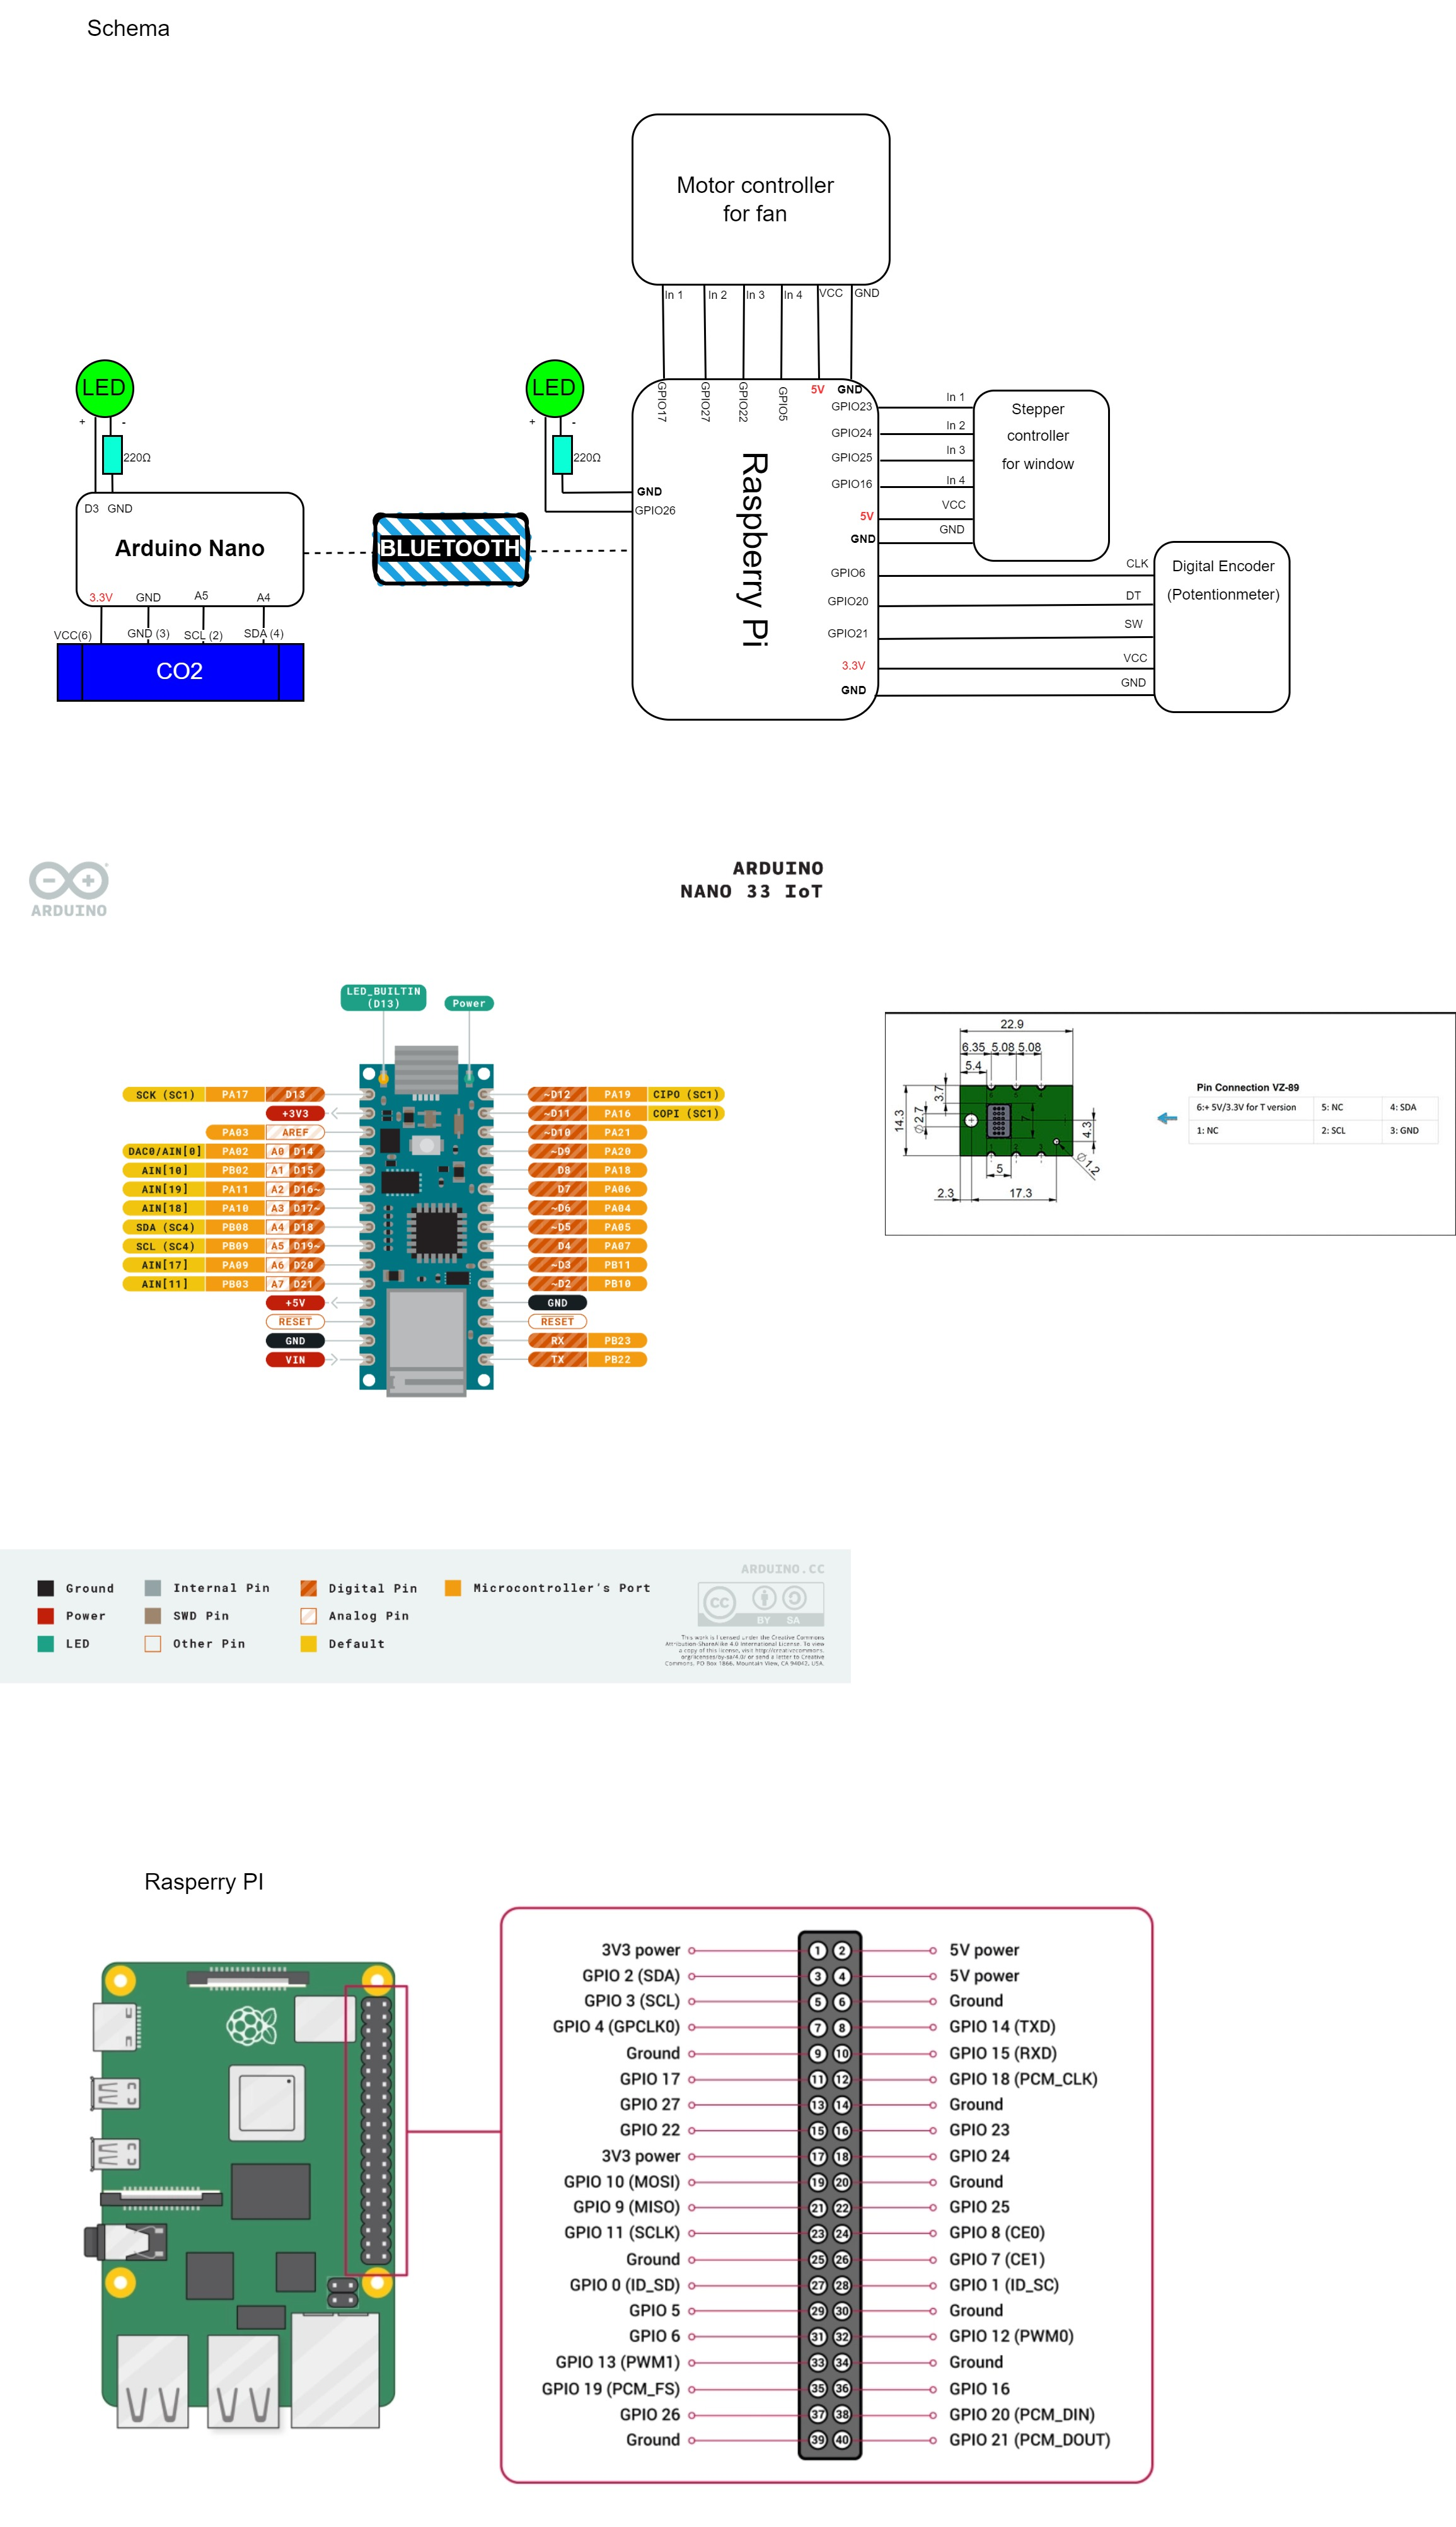
\includegraphics[height=200mm,left]{images/RoomVentilation_Cabling.jpg}
	\centering
	\caption{Arduino and Rasperry Pi}
	\label{fig:system}
\end{figure}